\section{Frontend}
\subsection{Mantine}

\subsubsection{Color scheme in plotly}
A minor addition to the \gls{gui} was to create a custom theme for \gls{plotly} that matched the graphic style of \gls{mantine}.
This can be seen in Figure \ref{fig:color_matching} where the colors in the plot are the same as the colors in the \gls{markdown} text below.

\begin{figure}[H]
    \centering
    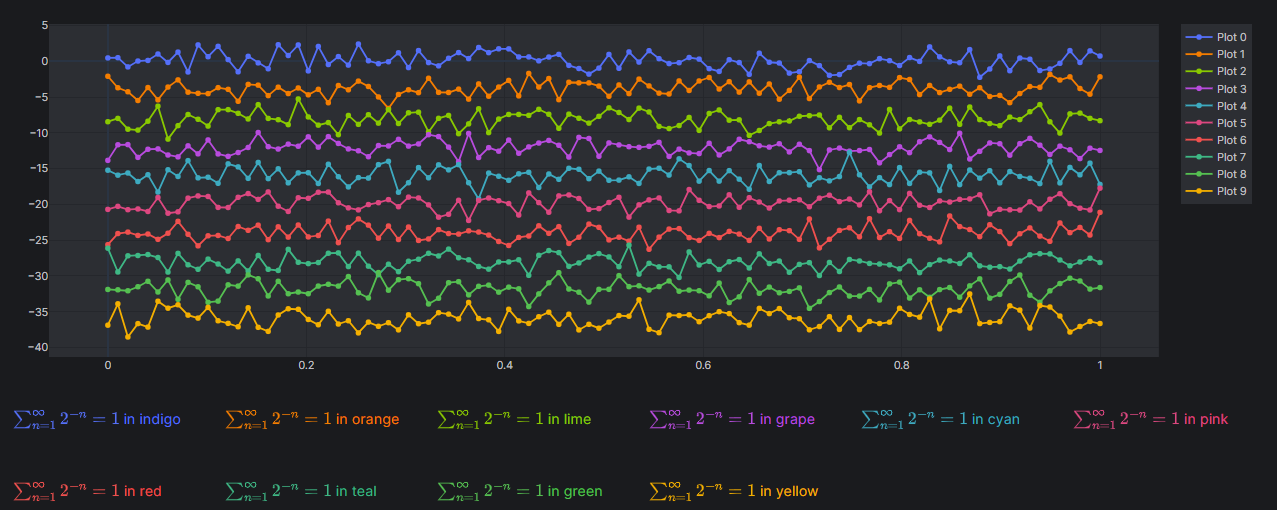
\includegraphics[width=\textwidth]{figures/gui/colors.png}
    \caption{Color matching between Plotly and Mantine}
    \label{fig:color_matching}
\end{figure}